The guarantees of CP can be applied to many different types of models. Different models, however, predict differently which may influence coverage and the prediction sets in practice. This influence may be significantly quantifiable.

CP can be extended by TODO TODO TODO. The performance is compared to TODO TODO TODO TODO

We will figure the TODO's out later

% 

\subsection{Behavior under different models}
Different model types trained on the same training data may have different prediction sets after application of CP and testing. The prediction sets can differ in both content and size, however, this difference may in practice be insignificant. This project will examine whether the prediction set size is significantly different between a convolutional neural network vs. a multinomial logistic regression model on a classification task on the EMNIST dataset.


\subsubsection{Models}
The logistic regression model is trained on the standardized, flattened feature vectors of each image. The model is implemented using the scikit learn logistic regression class with default arguments. The model therefore makes use of L2 regularization with a strength of $1$.

The trained convolutional neural network from \textit{Active Machine Learning and Agency - Bayesian Optimization on EMNIST} is reused. The CNN has $4$ convolution layers with a $3$×$3$
kernel, ReLU activation function; $4$ Max-pooling layers with a $2$×$2$ kernel. At the convolutional layer $i$, we set the number of feature maps to be $4 \cdot 2^i$. At the first convolutional layer, we then output $8$ feature maps. As the output layer, we have a single feed-forward layer before our output. The network was trained for $2$ epochs using a batch size of $200$ with a learning rate of $10^{-3}$ and a weight decay of $10^{-5}$. 

\begin{figure}
    \centering
    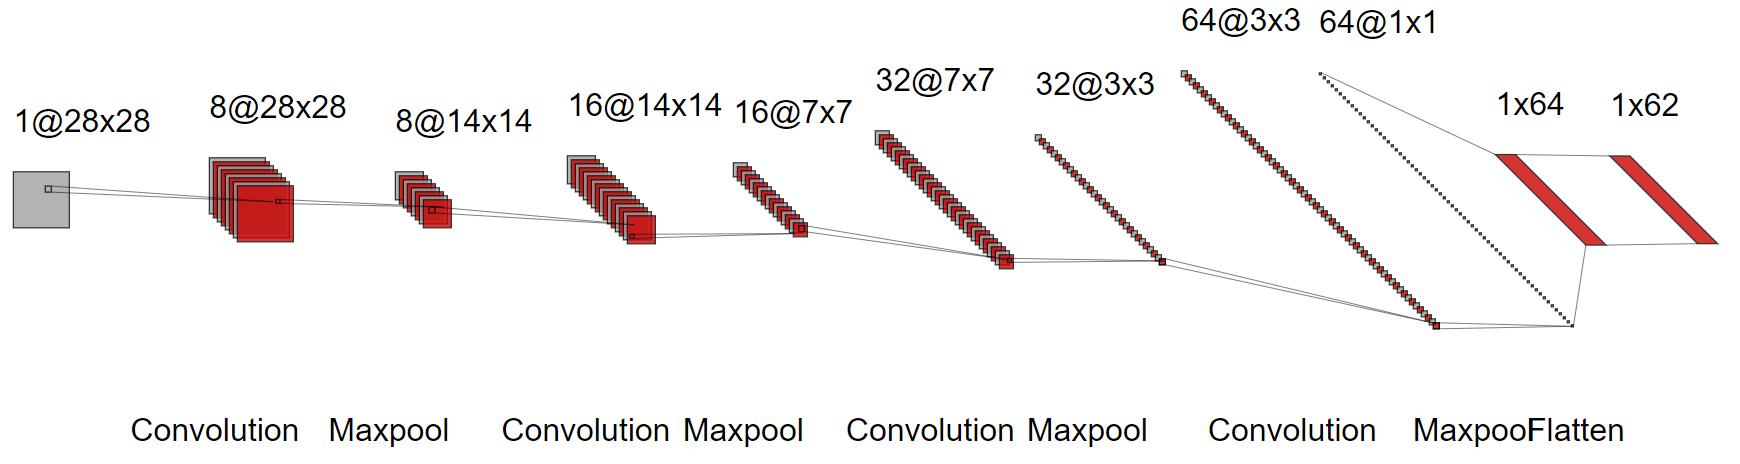
\includegraphics[width=0.8\textwidth]{Images/CNN_arch.png}
    \caption{Architecture of the convolutional neural network model}
\end{figure}


\subsubsection{Adaptive Conformal Prediction}
% The output probabilities of each model then have a conformal prediction framework applied on top. In this case a CP method called Adaptive Prediction Sets. The short description of this CP method is that it figures out how much of the output probability mass on average, $\hat{q}$, must be contained in the prediction set to gain coverage, and then it simply adds the classes with the highest probability mass to the prediction set until the required amount of probability mass has been obtained.
%
One framework for applying CP used in this report is called adaptive prediction sets. It is applicable for classification tasks, where the model outputs a probability distribution over the output classes, such as an ANN with softmax output or multinomial logistic regression.
The score function is then the cumulative sum of the probabilities in decreasing sorted order. That is, if $f_y(X)$ denotes the model output of the data point $X$ corresponding to the class $y$, then the score function is given by,
%
\begin{gather}
    s(X,y)=\sum_{i = 1}^k f_{\pi_i}(X), \quad \text{where $y = \pi_k$ and }k = \argmin_{i} [f_{\pi_i(X)} = f_y(X)]
\end{gather}
Here, $\pi_i$ is the class corresponding to the $i$'th largest model output. In case of ties, the last equality that defines $k$ means that we choose $k$ as small as possible.
% \begin{gather}
%     s(X,y)=\sum_{c\text{ :} f_c(X)\geq f_y(X)}f_c(X)
% \end{gather}
%
% Define $f_c(x)$ as the model's output probability for class $c$ on an image $x$. In addition, also define $f_{(-i)}(x)$ as the model's $i$'th highest output probability on an image $x$. Pay special attention to the parenthesis around $-i$, which denotes that it is an order statistic. The associated class for the second highest output probability would be $c_{(-2)}$. The score function is then given as:
% \begin{align*}
%     s(x, y) = \sum^{k}_{i=1} f_{c_{(-i)}}(x)
% \end{align*}
% Where $y$ is the class label for image $x$, and $k$ is given by $y = c_{(-k)}$.
%

In other words, sort all the output probabilities in descending order, and then sum them until the correct class is reached. This gives the score
% , $s$, for a prediction 
and it represents how much probability mass was required for the correct class to be included in the prediction set.
%
Then a procedure similar to the one described in the methods section is performed with $\hat q$ being the $\ceil{(n+1)(1-\alpha)}/n$ quantile of the calibration scores.
%and the prediction set defined as in \cref{eq: def. prediction set}
% The score is then calculated for the whole calibration set, and the quantile, $\hat{q}$, for some $\alpha$ is found as previously described. This quantile represents the amount of probability mass to include to gain marginal coverage. 

After the $\hat{q}$ has been found, a prediction set can be constructed as follows:
\begin{align*}
    \Tau(X) = \left\{ \pi_i, \ldots, \pi_k \right\}, ~\text{where}~ k = \text{inf}~ \left\{k' : \sum^{k'}_{i=1} f_{\pi_i}(X) \geq \hat{q} \right\}
\end{align*}
The equation says to include all the $k$ classes with the highest probability mass, such that the sum of the $k$ probability masses is above or equal to $\hat{q}$. The smallest possible $k$ where that is true is used.


\begin{figure}
    \centering
    \begin{subfigure}{0.44\textwidth}
        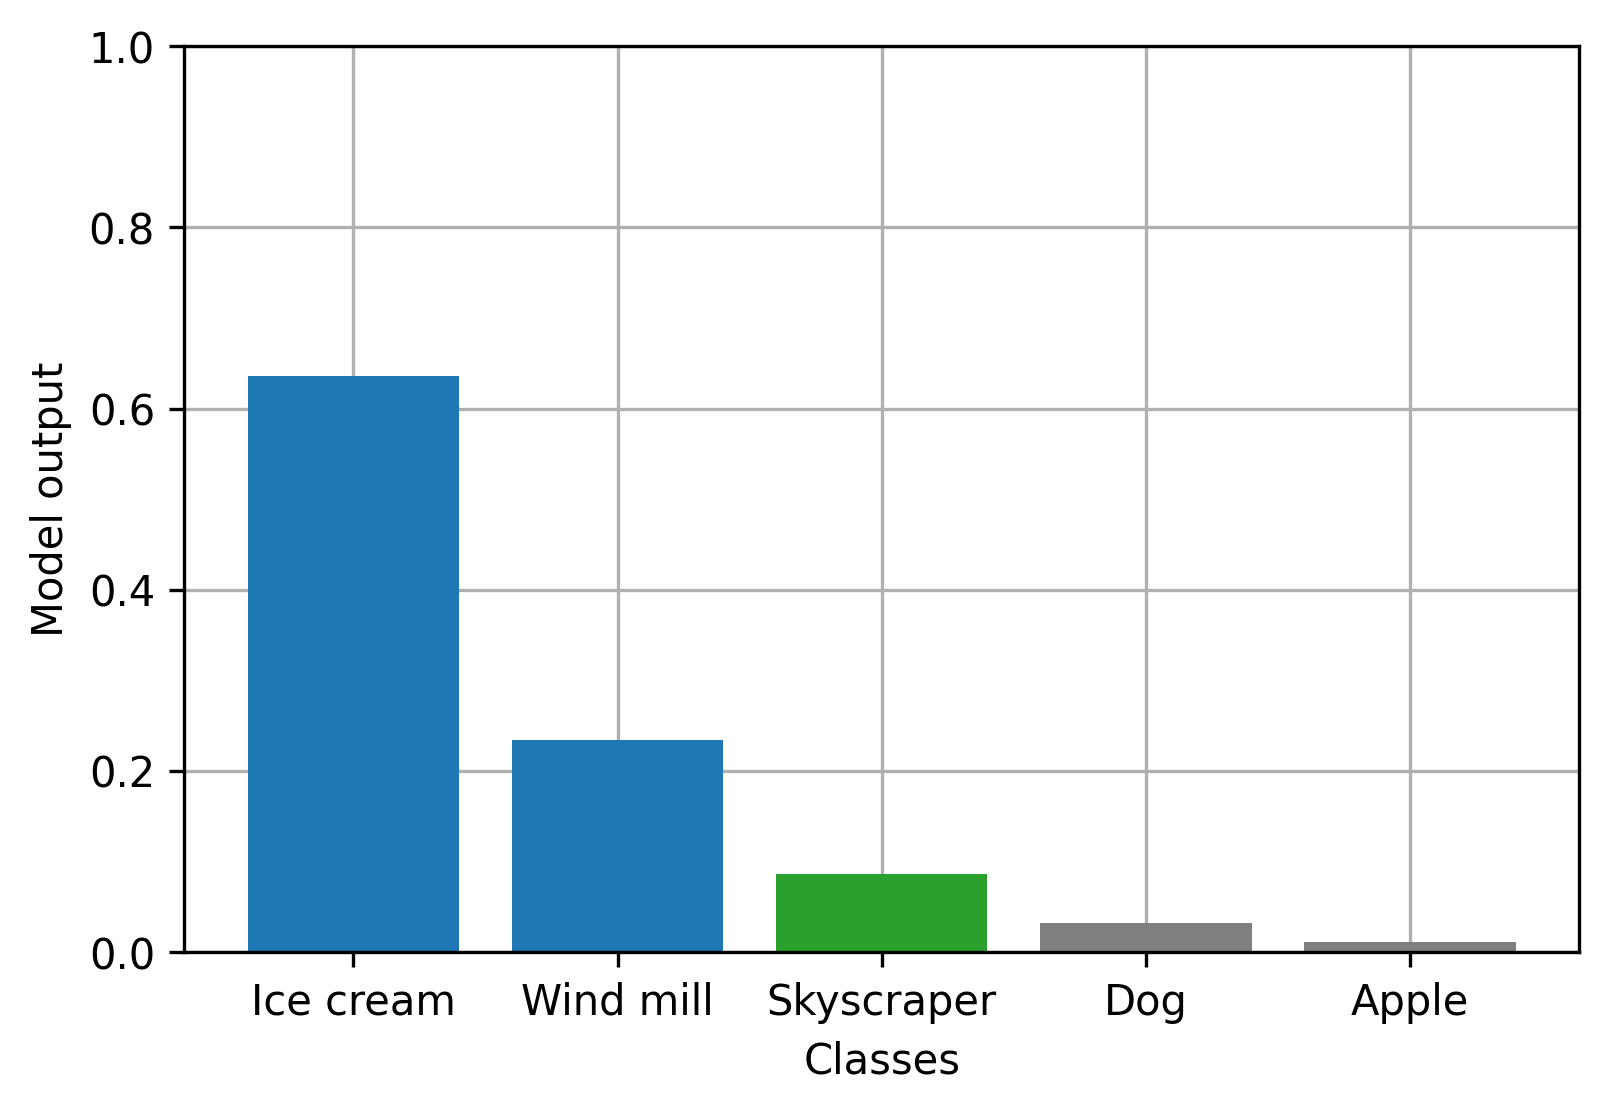
\includegraphics[width=\textwidth]{Images/adaptive-prediction-sets-score.png}
        \caption{Sorted model output for one image. The green class is the label for the image. The score is calculated as the sum of the probabilities of the blue and green classes.}
    \end{subfigure}
    \hspace{1em}
    \begin{subfigure}{0.44\textwidth}
        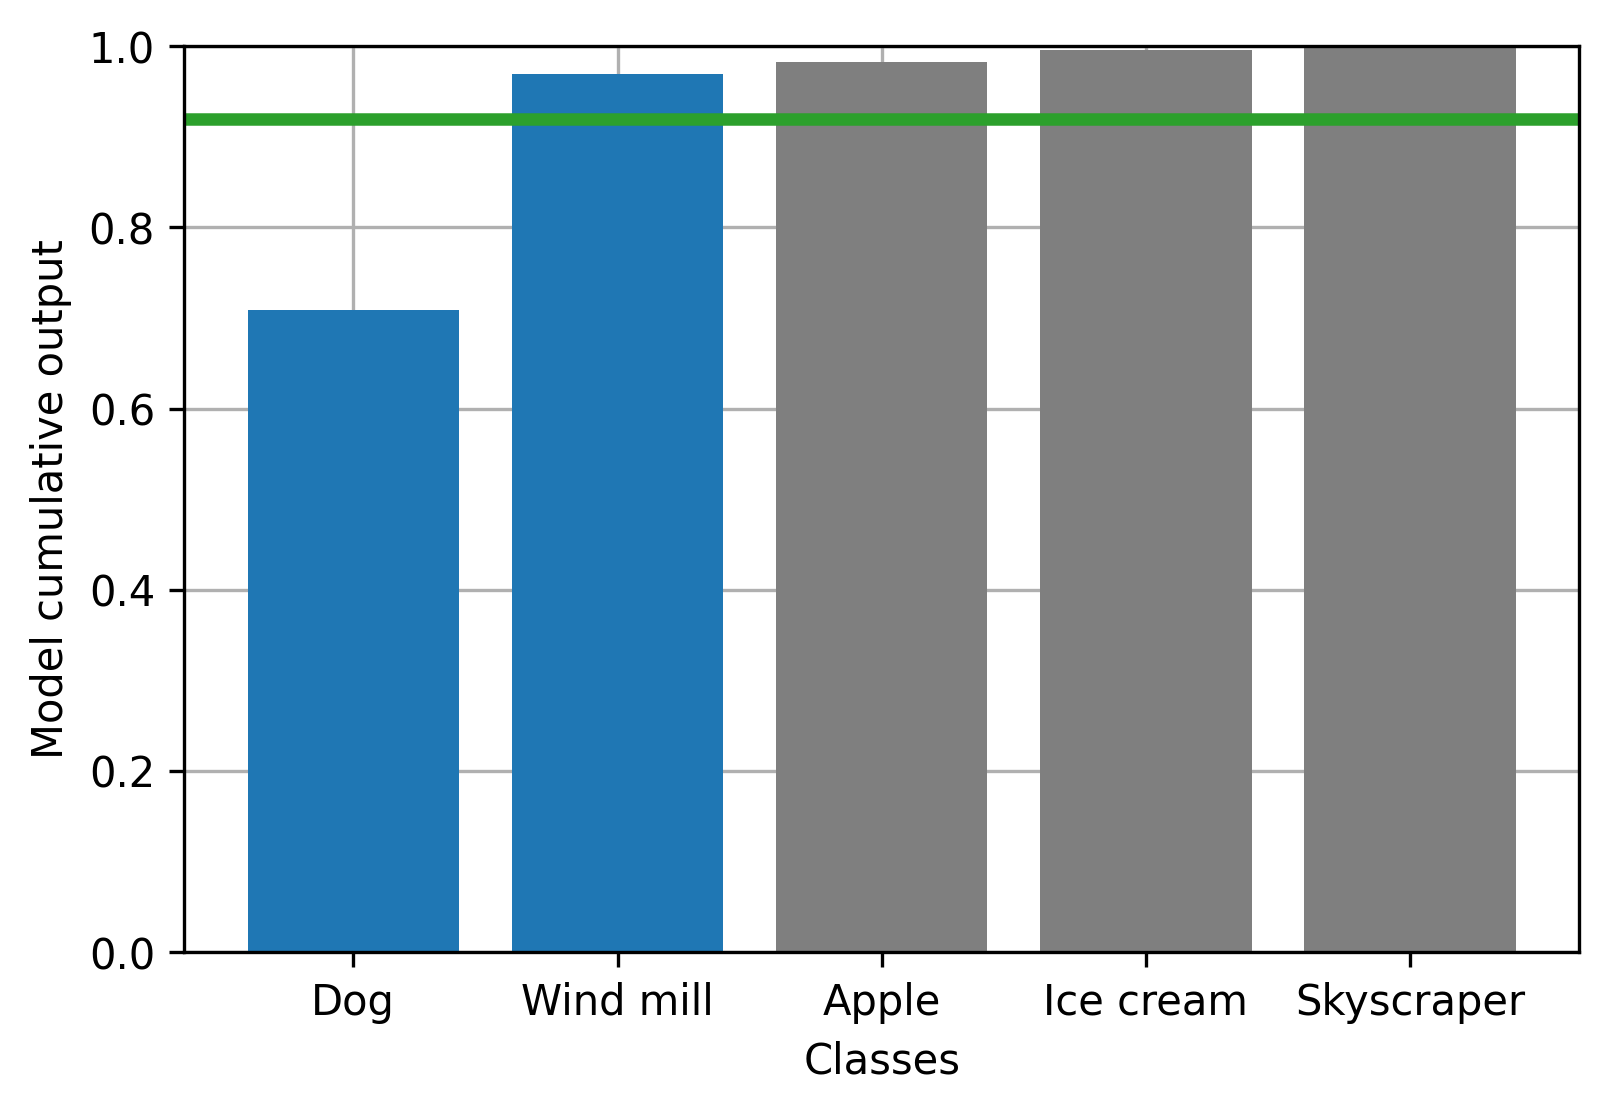
\includegraphics[width=\textwidth]{Images/adaptive-prediction-sets-prediction.png}
        \caption{Cumulative probability mass of sorted model output. The green line represents the quantile $\hat{q}$, while the blue classes represent the prediction set.}
    \end{subfigure}

    \caption{Visual example of calculations for Adaptive Prediction Sets. Note that the two figures come from different data points}
\end{figure}


\subsubsection{Evaluation}
A model with higher accuracy should naturally have smaller prediction sets on average with adaptive CP. Models with equivalent accuracy may, however, still differ in their prediction set sizes in that the distribution of the prediction set sizes may vary. 

Both models are trained on the same training data, calibrated on the same calibration data, and tested on the same test data. The prediction set size for each model for each test point is stored. Analysis is run on these pairs of prediction set sizes.

The prediction set size empirical densities are first plotted for each model and qualitatively evaluated. If the densities seem approximately normal and their variances seem approximately homogeneous, a paired t-test is used. The difference in prediction set sizes for test images is tested against the hypothesis of said difference being zero. If the densities appear to not be normally be distributed or have inhomogeneous variance - a Wilcoxon paired difference test is used in place of the paired t-test. If it turns out that no difference can be detected, a Kolmogorov-Smirnov test can in addition to a qualitative evaluation of the empirical densities be used to discuss the shape of the distribution.


\subsection{Extension of CP}
To be decided. Unable to write about for now.